% !TeX spellcheck = cs_CZ
\documentclass[FM,MP]{tulthesis}

\usepackage[utf8]{inputenc}
\usepackage[czech]{babel}
\usepackage{tul}
\usepackage[hidelinks,unicode,hyperfootnotes=false]{hyperref}
\usepackage{enumitem}
\usepackage{cite}

\linespread{1.3}

\TULtitle{Validace konfiguračních souborů Flow123d}{Validation of Flow123d configuration files}
\TULprogramme{N2612}{Elektrotechnika a informatika}{Electrical Engineering and Informatics}
\TULbranch{1802T007}{Informační technologie}{Information Technologies}
\TULauthor{Bc.~Tomáš Křížek}
\TULsupervisor{Jiří Vraný,~Ph.D.}
\TULyear{2015}
\TULid{M14000168}

\addto\captionsczech{\def\refname{Literatura}}

\begin{document}

\renewcommand{\thetable}{\arabic{table}}
\renewcommand{\thefigure}{\arabic{figure}}

\ThesisStart{male}

\begin{abstractCZ}
	Tento projekt se zabývá problematikou validace konfiguračních souborů Flow123d, jejichž struktura je dynamicky definována v závislosti na verzi Flow123d. V projektu jsou popsány specifika formátu konfiguračních souborů, jako jsou reference nebo automatické konverze. Dále je navržena datová struktura pro zpracování konfiguračních souborů a dynamicky definovaných datových typů. Součástí projektu je i dokumentace vytvořeného rozhraní.
\end{abstractCZ}
\vspace{2cm}
\begin{abstractEN}
	This project addresses the issues surrounding validation of Flow123d configuration files. Data structure of these files is dependent on the version of Flow123d. This paper describes the specifics of the configuration file format. These include references or automatic conversions. Next, a data structure for processing of configuration files and dynamycally defined data types is designed. The project also documents the created interface.
\end{abstractEN}

\tableofcontents
\clearpage

\chapter{Úvod}
	Tento projekt řeší problematiku validace konfiguračních souborů pro Flow123d. Software Flow123d\cite{bib:flow123d} slouží k simulaci toku podzemních vod a transportu látek nebo tepla. Konfigurační soubory mají dynamicky definovanou strukturu, která se liší podle verze Flow123d. Cílem je vytvořit nástroj, který určí, zda zadaný konfigurační soubor je validní pro danou verzi.

	Konfigurační soubory jsou ve formátu CON, který se podobá standardnímu formátu JSON. Od tohoto formátu se mírně odlišuje syntaxí. Konkrétní odlišnosti jsou popsány v kapitole \ref{format-con}. Kromě odlišné syntaxe také umožňuje vytvářet reference (viz kapitola \ref{reference}), se kterými je potřeba náležitě pracovat při zpracování dat. Formát CON také umožňuje v některých případech použít zkrácený zápis, který se poté čtečkou formátu automaticky zkonvertuje na požadovaný tvar. Problematikou automatických konverzí se zabývá kapitola \ref{automaticke-konverze}.

	Jelikož se struktura konfiguračních souborů se liší podle verze Flow123d, validace nespočívá pouze v ověření dat podle pevně daných pravidel. Pro validaci je nutné dynamicky načíst datové typy, které lze v rámci datové struktury použít. Sada těchto datových typů je dodána ve formátu JSON. Popis struktury konfiguračních souborů a možných datových typů je rozebrán v kapitole \ref{struktura-konf-souboru}.

	V kapitole \ref{implementace} se nachází dokumentace k vytvořenému rozhraní. Jsou zde popsány jednotlivé moduly, jejich funkčnost a použití. Také se zde nachází popis datových struktur pro reprezentaci obsahu konfiguračních souborů a jejich struktury.


\chapter{Formát konfiguračních souborů}
	\label{format-con}
	Konfigurační soubory, které je potřeba zvalidovat, jsou často psány ručně a nejsou strojově generovány. Formát CON, ve kterém jsou napsány, byl tomuto přizpůsoben. Syntaxe CON je podobná standardnímu formátu JSON, ale pro snažší zápis se mírně liší. Rozdíly v syntaxi oproti formátu JSON jsou následující.
	\begin{itemize}
		\item Klíče neobsahující mezeru mohou být napsány bez uvozovek.
		\item Klíč může být od hodnoty oddělen znakem \uv{\texttt{$=$}} místo \uv{\texttt{$:$}}.
		\item V souboru se mohou vyskytovat komentáře. Jsou povoleny víceřádkové komentáře uzavřené mezi sekvencemi \texttt{/*} a \texttt{*/}, nebo řádkové komentáře, které jsou uvozeny sekvencí \texttt{//}.
	\end{itemize}


	\label{semantika-con}
	Formát CON byl navržen pro inicializaci datových typů v C++. Kromě syntaktických rozdílů tedy předpokládá následující sémantická pravidla.
	\begin{itemize}
		\item Povolené datové typy jsou skalární hodnoty, pole nebo záznamy.
		\item Pole jsou vždy tvořeny prvky stejného typu.
		\item Záznam má určitý typ, který definuje seznam povolených klíčů.
		\item Každý klíč má daný typ, jméno a implicitní hodnotu.
		\item Klíče napsané velkými písmeny mají speciální význam a jsou zpracovány čtečkou CON formátu. Názvy ostatních klíčů jsou malými písmeny.
		\item U záznamů lze použít polymorfismus, kde klíč \texttt{TYPE} udává typ záznamu.
		\item Lze použít reference na data v rámci CON souboru pomocí speciálního klíče \texttt{REF}.
	\end{itemize}

	Bližší specifikace formátu CON lze nalézt v dokumentaci Flow123d\cite{bib:flow123d-manual}.


	\section{Reference}
		\label{reference}
		Formát CON umožňuje místo libovolné hodnoty, záznamu nebo pole uvést referenci na jiná data. Po načtení souboru je nutné tyto reference zpracovat tak, aby jejich chování odpovídalo referencím a nikoli pouhým kopiím. Pokud se tedy změní původní data, změní se i reference a naopak. Zpracování referencí by mělo proběhnout ihned po načtení souboru, tedy před automatickými konverzemi. 

		Reference jsou v konfiguračních souborech zapsány jako záznam, který obsahuje jediný klíč -- \texttt{REF}. V tomto klíčí je uvedena cesta, která určuje, na která data reference ukazuje. Cesta může být absolutní i relativní a ukazuje na libovolný uzel ve stromu. Pokud je součástí cesty záznam, v cestě je uveden klíč, který se vybere. Pro položky, které jsou součástí pole, se uvede jejich index (číslováno od 0). Pro oddělení úrovní ve stromu je použit znak \texttt{/}. 

		Reference mohou vypadat například následovně.
			\begin{itemize}
				\item \texttt{\{REF = "/system/output\_streams/0/format/TYPE" \}}
				\item \texttt{\{REF = "../../primary\_equation/solver" \}}
			\end{itemize}


	\section{Automatické konverze}
		\label{automaticke-konverze}
		Pro usnadnění psaní konfiguračních souborů existují určitá pravidla, která umožňují zkrátit zápis a vynechat některé údaje, které jsou poté doplněny automaticky. Existují dva typy automatických konverzí.

		První konverze proběhne, pokud se na vstupu očekává pole a místo něj se na vstupu nachází skalární hodnota nebo záznam. V tomto případě dojde k tomu, že se vytvoří pole s očekávanou dimenzí a do něj se vloží jediná položka -- hodnota, která je na vstupu.

		Druhá konverze proběhne, pokud je na vstupu pole nebo skalární hodnota místo záznamu. Tento záznam ale musí automatickou konverzi podporovat a to tím, že jeho definice obsahuje klíč \texttt{reducible\_to\_key}, který určuje, do kterého klíče v záznamu se má zapsat hodnota na vstupu. Ostatní hodnoty klíčů nabývají výchozích hodnot. Tato konverze funguje obdobně i pro abstraktní záznamy, které mají definované výchozího potomka. 

\chapter{Struktura konfiguračních souborů}
	\label{struktura-konf-souboru}
	Jak již bylo zmíněno v kapitole \ref{semantika-con}, data v konfiguračním soubor podléhají určitým sémantickým pravidlům. Uvedená pravidla jsou pouze obecná a jejich konkrétní podoba je závislá na verzi Flow123d. Požadavky na strukturu jsou popsány v dokumentaci Flow123d a pro potřeby aplikace je jejich specifikace dodána ve strojově čitelném formátu JSON.

	V této kapitole je popsán formát souboru specifikací. Nachází se v něm seznam datových typů, jejich popis, vlastnosti a struktura. Z jednotlivých položek lze vytvořit sada povolených datových typů, které lze použít v konfiguračním souboru. Každý datový typ má specifikované \texttt{id}, které ho jednoznačně identifikuje, a \texttt{input\_type}, který určuje základní datový typ, od kterého je daný typ odvozen. Základními datovými typy jsou skalár (viz tabulka \ref{tab:typy-skalaru}), pole (\textit{Array}), záznam (\textit{Record}) a abstraktní záznam (\textit{AbstractRecord}).

	Data v konfiguračním souboru tvoří stromovou strukturu. Pro jejich ověření se postupuje od kořene stromu k listům. Popis datového typu kořenu stromu je vždy uveden v seznamu jako první. Aby konfigurační soubor odpovídal dané specifikaci, musí být všechny uzly stromu validní. Pokud validní nejsou, zaznamená se, k jaké chybě došlo a kde.

	\begin{table}[h]
		\centering
		\caption{Datové typy skalárních hodnot}
		\label{tab:typy-skalaru}
		\begin{tabular}{|l|l|l|}
		\hline
		\textbf{Základní datový typ} & \textbf{Popis}           & \textbf{Pravidlo pro validaci}                                            \\
		\hline
		\textit{Integer}    & celé číslo      & hodnota musí být v rozmezí \texttt{min} a \texttt{max}               \\
		\textit{Double}     & desetinné číslo & hodnota musí být v rozmezí \texttt{min} a \texttt{max}               \\
		\textit{Bool}       & přepínač        & --                                                  \\
		\textit{String}     & řetězec         & --                                                  \\
		\textit{Selection}  & výběr z množiny & \parbox[t]{7cm}{musí obsahovat hodnotu z množiny povolených hodnot} \\
		\textit{FileName}   & cesta k souboru & --                                                  \\
		\hline
		\end{tabular}
	\end{table}

	\section{Skalární hodnoty}
		U skalárních typů spočívá validace v ověření správného datového typu a ověření validačního pravidla, pokud nějaké existuje. Pro číselné hodnoty se kontroluje rozmezí, které je určeno hodnotami \texttt{min} a \texttt{max} u specifikace datového typu. Speciální validaci vyžaduje také typ \textit{Selection}. U tohoto datového typu je dána množina povolených hodnot (\texttt{values}), kde každá hodnota má jméno (\texttt{name}), které ji jednoznačně identifikuje. Zadaná hodnota v \textit{Selection} je validní, pokud se shoduje se jménem některé z povolených hodnot.

	\section{Pole}
		Typ \textit{Array} má podobně jako číselné typy specifikované hodnoty \texttt{min} a \texttt{max}. U pole tyto hodnoty určují minimální, resp. maximální počet položek. Pravidlo pro validaci pole tedy spočívá v ověření počtu položek pole. Dále je nutné ověřit, zda jsou validní jednotlivé položky v poli. Pole jsou vždy homogenní, tedy všechny jeho položky jsou stejného typu, který je určen pomocí \texttt{subtype}.

	\section{Záznam}
		\label{struktura-zaznam}
		Typ \textit{Record} má unikátní jméno (\texttt{type\_name}) a obsahuje libovolný počet klíčů. Pokud je potomkem nějakých abstraktních záznamů, tak je jejich seznam uveden v položce \texttt{implements}. Položka \texttt{keys} definuje seznam povolených klíčů. V ní jsou dále uvedeny tyto položky:
		\begin{itemize}
			\item \texttt{key}: definuje název klíče,
			\item \texttt{description}: popis klíče,
			\item \texttt{type}: typ klíče,
			\item \texttt{default}: obsahuje dále \texttt{type}, který určuje typ výchozí hodnoty a \texttt{value} implicitní hodnotu.
		\end{itemize}

		Typ defaultní hodnoty může nabývat hodnot \textit{obligatory}, \textit{value at declaration}, \textit{value at read time} a \textit{optional}. Pro potřeby validace je důležitá pouze hodnota \textit{obligatory}, která specifikuje, že klíč musí být v záznamu uveden. Všechny ostatní typy klíčů nemusí být v záznamu uvedeny. Validace záznamů spočívá v ověření, zda jsou přítomny všechny klíče, které jsou povinné (\textit{obligatory}), a dále v ověření typu všech klíčů, které jsou v záznamu uvedené.

	\section{Abstraktní záznam}
		Speciální typ záznamu, který umožňuje polymorfismus, je \textit{AbstractRecord}. Obsahuje položku \texttt{implementations}, ve které jsou uvedeny všechny zázamy, které ho implementují. Další důležitou položkou je \texttt{default\_descendant}. Pokud je uvedena, tak definuje výchozí typ záznamu.

		Při validaci záznamu je nutné nejprve určit jeho typ. K tomu slouží klíč \texttt{TYPE}, který je přímo uveden u daného záznamu v konfiguračním souboru. Pokud tento klíč není uveden, použije se typ, který je určen pomocí \texttt{default\_descendant}. Pokud ani takto nelze určit typ záznamu, jedná se o chybový stav. Po určení typu záznamu se provede validace podĺe pravidel, které definuje přímo konkrétní datový typ. 

\chapter{Implementace}
	\label{implementace}
	Aplikace pro validaci byla vytvořena v jazyce Python verze 3. Detaily a použití tohoto jazyka je popsáno na webových stránkách s jeho dokumentací\cite{bib:python}. Vytvořená aplikace se skládá z několika modulů, jejichž propojení je znázorněno na obrázku \ref{img:propojeni-modulu}.

	\begin{figure}[h]
		\centering
		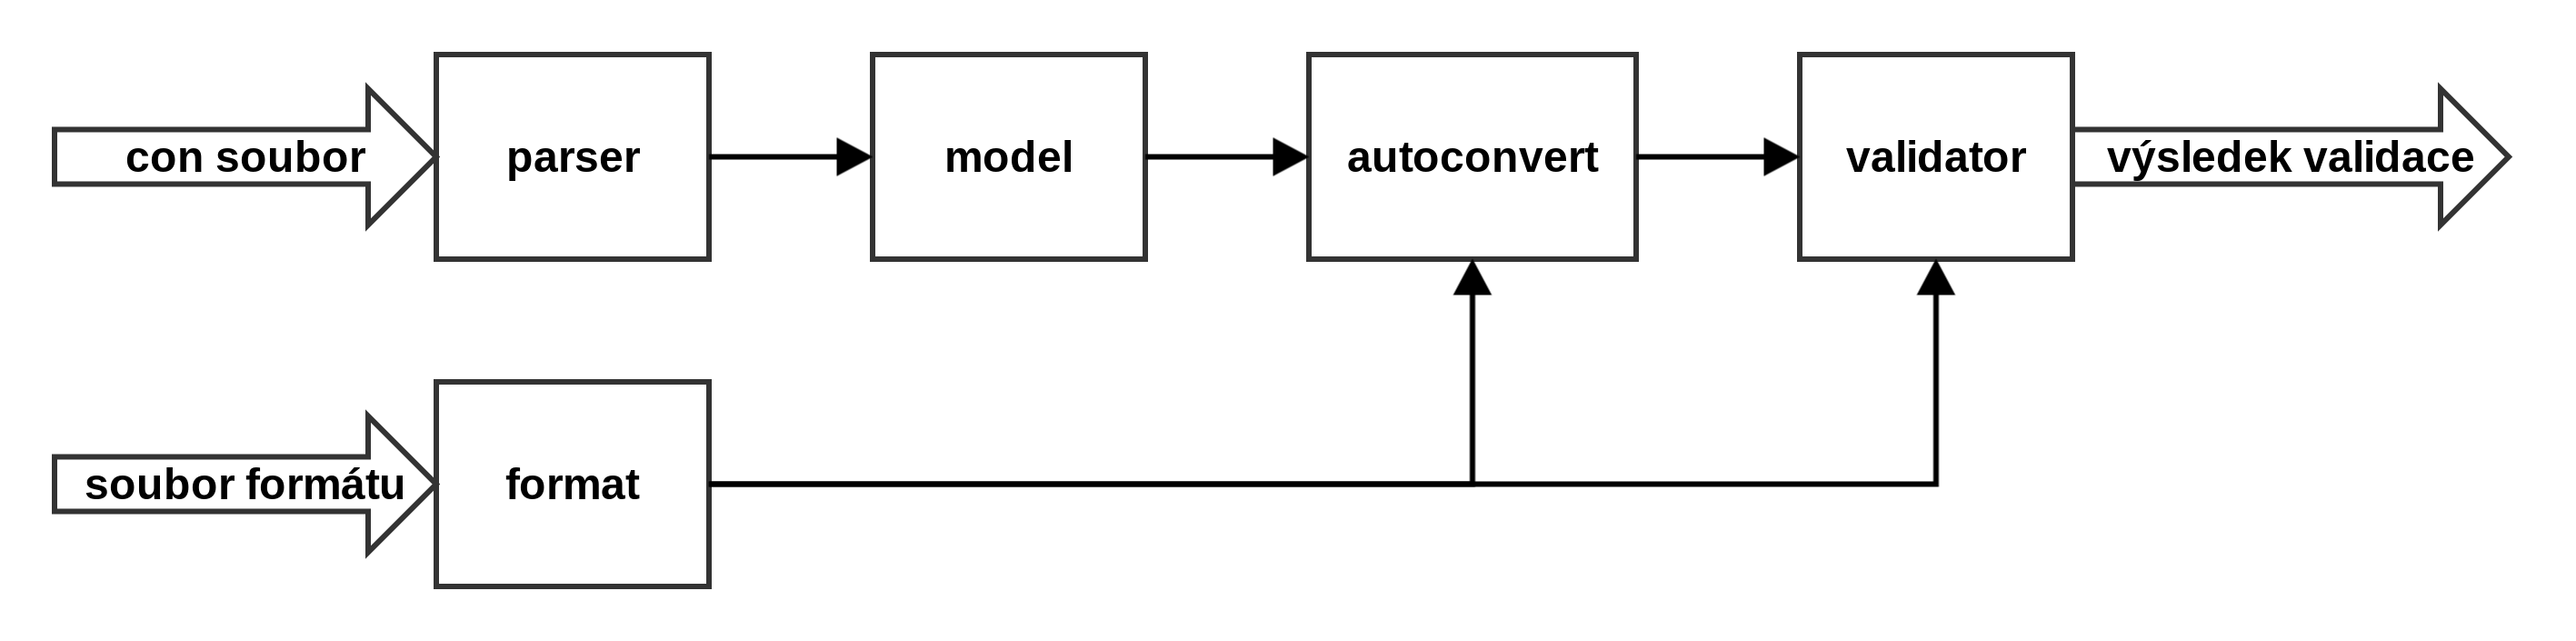
\includegraphics[width=\linewidth]{../img/con_modules.png}
		\caption{Propojení modulů}
		\label{img:propojeni-modulu}
	\end{figure}

	Vstupem do aplikace jsou dva soubory. Jedním z nich je samotný konfigurační soubor, na obrázku uveden jako \textit{con soubor}. Druhým z nich je soubor, který obsahuje kompletní popis konkrétní verze formátu, tedy výčet všech možných datových typů, jejich strukturu a uspořádání, na obrázku je uveden jako \textit{soubor formátu}. Výstupem z aplikace je informace, zda konfigurační soubor odpovídá danému formátu, tedy jestli je validní, případně informace o nalezených odlišnostech.

	Přečtení souboru a vytvoření jeho datové reprezentace zajišťuje modul \texttt{parser}. Vstupem do tohoto modulu je cesta ke konfiguračnímu souboru. Modul tento soubor načte, interpretuje a vytvoří jeho datovou reprezentaci s pomocí modulu \texttt{model}.

	Modul \texttt{format} zajišťuje načtení souboru formátu, který obsahuje popis a propojení použitelných datových typů. Výstupem z tohoto modulu je specifikace formátu \texttt{InputTypeSpec}, která reprezentuje datový typ kořenového prvku ve stromové struktuře, kterou data tvoří.

	Modul \texttt{autoconvert} provede v modelu automatické konverze. Aby bylo možné konverze provést, je potřeba kromě samotného modelu dodat tomuto modulu i očekávaný formát souboru.

	Modul \texttt{validator} očekává na vstupu model, ve kterém již proběhly automatické konverze, a formát souboru. Modul ověří, zda dodaný model je v očekávaném formátu.

	Následuje popis jednotlivých modulů a jejich veřejných funkcí, tříd a metod.

	\section{Modul \texttt{model}}

		\subsection*{\texttt{DataNode}}
			Třída reprezentuje jednotlivé uzly, které jsou součástí datového stromu. Obvykle se pracuje s kořenem stromu, ze kterého je možné se dostat k libovolnému jinému uzlu.

			\subsubsection{Atributy}
				\begin{itemize}[leftmargin=2cm]
					\setlength\itemsep{-2mm}
					\item[\texttt{value}] dle typu uzlu obsahuje buď přímo hodnotu, nebo potomky ve formě seznamu nebo slovníku. Potomci jsou opět typu \texttt{DataNode}. Pokud je nastavena \texttt{ref}, vrací se \texttt{value} reference.
					\item[\texttt{ref}] umožňuje nastavit referenci na jiný objekt typu \texttt{DataNode}. Ve výchozím stavu obsahuje hodnotu \texttt{None}.
					\item[\texttt{path}] vrací absolutní cestu k tomuto uzlu ve stromu.
					\item[\texttt{its}] \textit{nepovinný}; určuje \texttt{InputTypeSpec} (viz kapitola \ref{input-type-spec}) tohoto uzlu
				\end{itemize}
			
			\subsubsection{Metody}
				\paragraph{\texttt{DataNode(data, [parent, [name]])}}
					inicializuje třídu podle argumentu \texttt{data}. Pokud se jedná o stromovou strukturu, která je tvořena slovníky a seznamy, dojde rekurzivně k vytvoření celého stromu a tato třída je kořenem celého stromu. Volitelné atributy \texttt{parent} a \texttt{name} mají využití především pro inicializaci potomků ve stromové struktuře, kdy \texttt{parent} specifikuje nadřazený uzel a \texttt{name} udává název uzlu, který se použije při generování cesty ve stromu.
				\paragraph{\texttt{get(path)}}
					interpretuje zadanou cestu \texttt{path} a vrátí uzel na dané cestě ve stromu, pokud existuje. V opačném případě se vyvolá výjimka \textit{LookupError}.

	\section{Modul \texttt{format}}
		\subsection*{\texttt{InputTypeSpec}}
			\label{input-type-spec}
			Třída reprezentuje konkrétní datový typ, který se může vyskytnout na vstupu. Obsahuje všechna omezení a pravidla, která jsou potřeba pro validaci tohoto datového typu. Obdobně jako data tvoří stromovou strukturu a obvykle se tak pracuje s kořenovým typem, který popisuje kompletní strukturu dat.
			\subsubsection{Atributy}
				Existence jednotlivých atributů je závislá na základním datovém typu, z kterého je tento typ odvozen.
				\begin{itemize}[leftmargin=4cm]
					\setlength\itemsep{-2mm}
					\item[\texttt{id}] unikátní identifikátor datového typu
					\item[\texttt{input\_type}] základní datový typ, ze kterého je tento typ odvozen (možné typy viz kapitola \ref{struktura-konf-souboru})
					\item[\texttt{name}] \textit{nepovinný}; název datového typu pro generování dokumentace
					\item[\texttt{full\_name}] \textit{nepovinný}; úplný název datového typu pro generování dokumentace
					\item[\texttt{description}] \textit{nepovinný}; popis datového typu pro generování dokumentace
					\item[\texttt{min}] pro \textit{Integer}, \textit{Double}, \textit{Array}; udává minimální hodnotu, resp. minimální počet prvků
					\item[\texttt{max}] pro \textit{Integer}, \textit{Double}, \textit{Array}; udává maximální hodnotu, resp. maximální počet prvků
					\item[\texttt{values}] pro \textit{Selection}; slovník obsahující možné hodnoty, každá hodnota má název (\texttt{name}) a popis (\texttt{description})
					\item[\texttt{file\_mode}] pro \textit{FileName}; určuje zda-li je soubor pro čtení/zápis
					\item[\texttt{subtype}] pro \textit{Array}; určuje \texttt{InputTypeSpec} položek v poli
					\item[\texttt{type\_name}] pro \textit{Record}; unikátní název datového typu záznam
					\item[\texttt{type\_full\_name}] pro \textit{Record}; úplný unikátní název datového typu záznam
					\item[\texttt{keys}] pro \textit{Record}; obsahuje popis klíčů záznamu (viz kapitola \ref{struktura-zaznam})
					\item[\texttt{implements}] \textit{nepovinný}, pro \textit{Record}; určuje, který \textit{AbstractRecord} tento záznam implementuje
					\item[\texttt{reducible\_to\_key}] \textit{nepovinný}, pro \textit{Record}; určuje, který klíč se má použít při automatocké konverzi (viz kapitola \ref{automaticke-konverze})
					\item[\texttt{implementations}] pro \textit{AbstractRecord}; slovník obsahující \texttt{type\_name} a \texttt{InputTypeSpec}, které implementují tento abstraktní typ
					\item[\texttt{default\_descendant}] \textit{nepovinný}, pro \textit{AbstractRecord}; výchozí \texttt{InputTypeSpec}, který se použije, pokud není uveden jiný datový typ
				\end{itemize}
		\subsection*{\texttt{parse\_format(filename)}}
			Funkce přečte soubor s cestou \texttt{filename} a vrátí kořenový datový typ \texttt{InputTypeSpec}.

	\section{Modul \texttt{autoconvert}}
		\subsection*{\texttt{convert(node, [its])}}
			Funkce provede automatické konverze (viz kapitola \ref{automaticke-konverze}) na vstupních datech \texttt{node}. Funkce rekurzivně prochází vstupní strom, proto se volá se pro kořen stromu. Pokud není uveden datový typ \texttt{its}, použije se datový typ uzlu \texttt{node.its}.


	\section{Modul \texttt{validator}}
		\subsection*{\texttt{Validator}}
			Třída slouží pro validaci vstupních dat podle zadaného formátu. Kromě určení, zda jsou data validní, umožňuje identifikovat detekované odlišnosti od požadovaného formátu.

			\subsubsection{Atributy}
				\begin{itemize}[leftmargin=3cm]
					\setlength\itemsep{-2mm}
					\item[\texttt{errors}] seznam obsahující uzly (\texttt{DataNode}), ve kterých došlo k chybě, a příslušné výjimky (\texttt{Exception}), které nastaly
					\item[\texttt{console\_log}] vrací řetězec, který obsahuje zformátovaný text pro výpis chyb do konzole
				\end{itemize}
			
			\subsubsection{Metody}
				\paragraph{\texttt{validate(node, [its])}}
					Metoda určí, zda uzel \texttt{node} odpovídá formátu \texttt{its}. Vrací \textit{True} nebo \textit{False}, podle toho, zda uzel odpovídá danému formátu. Pokud není uveden formát \texttt{its}, použije se \texttt{node.its}. Po zavolání této metody je možné získat výjimky, ke kterým došlo při validaci, pomocí atributu \texttt{errors}. Proces validace probíhá tak, jak byl popsán v kapitole \ref{struktura-konf-souboru}.


	\section{Modul \texttt{parser}}
		\subsection*{\texttt{parse\_con(filename)}}
			Funkce přečte soubor s cestou \texttt{filename} a vrátí datovou reprezentaci vstupního CON souboru. Při načítání souboru je využit balík demjson\cite{bib:demjson}. Funkce zároveň vytvoří příslušné reference, které byly zadány pomocí klíče REF, tak jak bylo popsáno v kapitole \ref{reference}.

			Výstupem z funkce je kořen (\texttt{DataNode}) načtené datové struktury. Jedná se pouze o reprezentaci dat z konfiguračního souboru, která jsou nezávislá na očekávaném formátu. Oproti tomu data, která projdou automatickou konverzí, jsou již závislá na konkrétním formátu.

\chapter{Závěr}
	V rámci projektu bylo vytvořeno funkční rozhraní pro ověření konfiguračních souborů pro program Flow123d, které mají v různých verzích odlišnou strukturu. Aplikace podporuje speciální vlastnosti formátu CON, jako jsou reference nebo automatické konverze.

	Pro potřeby aplikace byla vytvořena datová struktura pro reprezentaci obsahu konfiguračních souborů. Některé její vlastnosti byly navrženy s ohledem na budoucí použití, které je popsáno dále.

	Součástí aplikace je i datová struktura pro popis struktury formátu, který je určen dynamicky podle verze Flow123d. Vytvořená datová struktura umožňuje načíst libovolnou verzi formátu a přizpůsobit jí proces validace. Datová struktura pro popis formátu bude dále použita generování nápovědy a dokumentace v aplikaci GeoMop.

	Vytvořené rozhraní má být jednou ze součástí nově vznikající aplikace GeoMop, která bude sloužit uživatelům aplikace Flow123d. Načtení a validace datové struktury bude součástí kontextu Model, který bude umožňovat práci s různými verzemi konfiguračních souborů.

	Navržený validátor umožní ověřit data, která uživatel zadá v grafickém rozhraní. Jeho hlavní funkcí a přínosem je však určení verze formátu konfiguračního souboru. Na základě ověření, zda data odpovídají odlišným verzím formátu, bude možné určit správnou verzi formátu souboru a případně tento soubor zkonvertovat na formát jiné verze.

\clearpage

\begin{thebibliography}{99}
	\addcontentsline{toc}{section}{\refname}
	
	\bibitem{bib:flow123d}
		Flow123d [online]. 2015. [cit. 2015-05-11]. Dostupné z: \url{http://flow123d.github.io/}
		
	\bibitem{bib:flow123d-manual}
		BŘEZINA, Jan, Jan STEBEL, David FLANDERKA, Pavel EXNER a Jiří HNÍDEK. 2015. \textit{Flow123d} [online]. Liberec [cit. 2015-05-11]. Dostupné z: \url{http://bacula.nti.tul.cz/~jan.brezina/flow123d_packages/1.8.2_release/flow123d_1.8.2_doc.pdf}. Documentation of file formats and brief user manual. Technical university of Liberec.

	\bibitem{bib:python}
		PYTHON SOFTWARE FOUNDATION. \textit{Python 3.4.3 documentation} [online]. 2015 [cit. 2015-05-14]. Dostupné z: \url{https://docs.python.org/3/}
		
	\bibitem{bib:demjson}
		MERANDA, Deron. Demjson and jsonlint. \textit{Python: module demjson} [online]. 2014 [cit. 2015-05-13]. Dostupné z: \url{http://deron.meranda.us/python/demjson/}
	
\end{thebibliography}

\end{document}